\documentclass[UTF8, oneside, fontset=mac]{pkuthss}
\usepackage[backend = biber, style = gb7714-2015ay,doi=false, url=false]{biblatex}
\usepackage{longtable,multirow,booktabs}
\usepackage{float,caption}
\usepackage{fontspec}
\usepackage{rotating}
\usepackage[perpage]{footmisc}
% \usepackage{amsmath,amssymb,amsthm}
\newtheorem{hyp}{假设}
% \aboverulesep=0ex
% \belowrulesep=0ex
\usepackage{arydshln}
\newif\ifblind\blindfalse
\renewcommand*{\bibfont}{\zihao{5}\linespread{1.27}\selectfont}
% \renewcommand{\thefootnote}{\@arabic\c@footnote}
\setlength{\bibitemsep}{3bp}
\newif\ifblind\blindfalse
\pkuthssinfo{
	cthesisname = {硕士学位论文}, ethesisname = {Master Thesis},
	thesiscover = {硕士学位论文},degreetype={2},
	ctitle = {极端天气冲击对风险偏好的影响——以家财险需求为例},
	etitle = {The Impact of Extreme Weather Shock on Household Property Insurance Demand},
	cauthor = {董晨阳}, eauthor = {Chenyang Dong}, date = {\today},
	studentid = {2201211201}, school = {经济学院},
	cmajor = {保险学}, emajor = {Insurance},
	direction = {保险学}, mentorlines = {1},
	cmentor = {刘新立},
	ementor = {Xinli Liu},
	ckeywords = {极端天气;风险偏好;家财险需求;保险市场},
	ekeywords = {Extreme Weather; Risk Preferences; Home Property Insurance Demand; Insurance Market},
}
\addbibresource{thesis.bib}
\hypersetup{
    hidelinks,
}
\begin{document}
\frontmatter
\pagestyle{empty}
\ifblind\makeblind\else\maketitle\fi
% \clearpage
\include{chap/copy}
\clearpage
\pagestyle{plain}
\setcounter{page}{0}
\pagenumbering{Roman}
%!TEX root = ../thesis.tex
\begin{cabstract}
\end{cabstract}
\begin{eabstract}
\end{eabstract}

\tableofcontents
\mainmatter
%!root = ../main.tex
% 极端气候定义、风险偏好=>风险厌恶程度、家财险定义
\chapter{引言}
\section{研究背景与意义}

2023年10月24日,我国政府宣布增发2023年国债1万亿元,集中用于灾后恢复重建和提升国家防灾减灾能力。这一决策表明政府对气候变化带来的灾害风险的高度关注,也突显了防灾减灾工作的紧迫性。在现代社会,气候变化已经成为一个备受瞩目的全球性问题。随着极端气候事件的频繁发生,人们对自身及财产的安全日益关切。在灾害面前,家庭往往是首当其冲的受害者。但与企业相比,个人家庭对这些潜在风险的反应可能更为复杂。家庭是否会通过购买家财险来缓解财产损失,以及他们在灾害发生后是否更加倾向于购买保险,这些问题有许多影响因素,具有较强的实证研究价值。

我国的家财险始于1980年,是当时中国人保重点推广的基础险种之一。在1980年,全国范围内有34200户家庭购买了中国人保的家财险,承保金额为5232万元,保费仅为7万元,仅占国内产险保费总额的0.02\%。到了1989年,全国家财险(包括储蓄性两全险)的投保户数增至76,910,000户,承保金额达1974亿元,保费收入为3.2亿元,占产险保费总额的4.4\%。可以说,我国财产保险的早期发展同时也是家庭财产保险演进的历史\citep{黄英君2008论我国产险公司分散性业务营销模式的创新},塑造了国人对财产险最早的认知。
% 然而,随着汽车保有量的急剧增加,财产险公司主要将注意力集中在车险上,导致车险成为财产险中的绝对主导领域,而家财险逐渐被边缘化,稳定增长长期不被关注。
% 我国家财险近十年保费收入持续提升,市场蓬勃发展但仍与发达国家有所差距。在2013-2021年家财险保费收入从38亿逐步提升至98亿后,2022年家财险以67.22\%的增长率成为了保费增速最快的产险险种,保费达到164亿,但家财险2022年末在行业保费规模中占比仅1.1\%。由于我国城市住宅建筑结构抗风险能力高,对于自然灾害风险暴露较低,因而我国住户对于风险感知度较低,对于保险产品的认知更为有限,保险深度也偏低,存在较大的保障缺口,商业化进展任重而道远。对比国外,美国家财险覆盖率为85\%\citep{croll2018home},2022年市场规模为1483亿美金,约合1.05万亿人民币;日本覆盖率达82\%\citep{plaza},2022年市场规模为1.2万亿日元,约合500亿人民币。可以看出,我国家财险市场仍有较大的发展空间。
% % https://mp.weixin.qq.com/s/4PTD5xrrEyDIuoBtbip2sQ
% \begin{figure}[H]
%     \centering
%     \includegraphics[width=\linewidth]{img/家庭财产保险保费.png}
%     \caption{家财险保费持续增长}
% \end{figure}

近年来,极端天气事件也层出不穷。据统计,全球范围内的极端天气事件频率和强度都在不断增加。这些极端天气事件包括暴雨、洪水、干旱、飓风等,给人们的生活和财产带来了巨大的风险和损失。巨灾频繁发生给人们造成物质上的创伤同时,也对人们的风险偏好有着潜移默化的影响,例如位于台风路径上的企业更偏好持有现金\citep{杨娜娜2019自然灾害与企业现金持有}。极端天气冲击对人们风险偏好是否会产生影响以及产生何种影响是一个值得研究的课题,能帮助我们提前做好风险管理措施,而不是总是亡羊补牢。

\begin{table}[H]
    \centering
    \caption{今年来全球极端天气}
    \begin{tabular}{lll}
        \toprule
        事件       & 时间                    & 死亡人数                            \\
        \midrule
        丹尼尔风暴    & 9月4日–12日              & \textgreater{}4,034+(10,100+失踪) \\
        弗雷迪飓风    & 2月5日–3月14日            & 1,434                           \\
        摩卡飓风     & 5月9日–15日              & 438(+101失踪)                     \\
        阿富汗寒潮    & 1月10日–17日             & 166                             \\
        西北美洲热浪   & 5月–至今                 & \textgreater{}112               \\
        北印度洪水    & 7月10日–至今              & \textgreater{}100               \\
        菲律宾洪水    & 2022年12月18日–2023年2月5日 & 97(+25失踪)                       \\
        圣保罗洪水和滑坡 & 2月18日–23日             & 65(+58失踪)                       \\
        巴基斯坦洪水   & 6月22日–7月6日            & 54                              \\
        奥蒂斯飓风    & 10月22日–25日            & 50–350                          \\
        \bottomrule
    \end{tabular}
\end{table}

然而,极端天气下人们对自身及财产安全的关切是否能够持续转化为对保险的需求,尤其是在家庭层面,却是一个相对较少被深入研究的领域。过去的国内研究主要关注气候变化对企业财产险或健康险的影响,比如雾霾天导致大量健康险投保之后又退保等,但是对于家庭财产保险的定量研究却相对较少。本研究的选题来源于对这一领域的关注,力图深入了解极端天气极端冲击对风险偏好的影响,填补现有研究的空白。

在此背景下,我们将通过深入研究极端天气对家财险需求的影响,探索个人家庭在面对气候变化时的风险管理行为,为保险业和政策制定提供更为全面的了解。本研究的意义不仅仅停留在学术探究层面,更涉及到实际社会和经济层面的多个方面:

首先,通过深入研究极端天气对家财险需求的影响,我们能够为保险公司提供更为精准的市场预测。这对于保险公司的产品开发、定价和风险管理具有重要指导意义。预测气候事件可能引发的家财险需求波动,可以帮助保险公司制定更灵活的营销策略,及时调整产品组合,提高市场适应性。

其次,研究结果还可以为政府和监管机构提供政策制定的依据。随着极端天气对保险市场的影响逐渐显现,相关的监管政策也需要跟进。通过深入了解家庭在面对气候变化时的保险需求变化,政府可以更好地制定相关政策,促进保险市场的健康发展,确保公众的保险保障能力。

此外,研究家财险需求的变化还能够提供社会科学领域对于人类行为和决策的深刻洞察。了解在灾害面前个体的风险认知和行为模式,有助于拓展对人类在危机时刻的心理和社会反应的认知。这对于制定个体和社会层面的应对策略,以及心理健康服务的提供都具有积极的实践意义。

最后,从可持续发展的角度来看,本研究有助于引导人们更加理性和科学地对待气候变化风险。通过了解保险在气候变化应对中的作用,可以提高社会对于个体责任和社会共担责任的认识。这有助于形塑一种更加可持续、共同应对气候挑战的社会文化氛围。

\section{文献综述}

本文主要从两个角度梳理国内外相关文献:一是气候变化对不同保险需求的影响,二是风险偏好的影响因素。

\subsection{极端天气冲击对不同种类保险需求的影响}
一般认为极端天气是指气象要素的极端值,包括极端温度、极端降水、极端风速、极端湿度、极端干旱等\citep{傅良2022ECMWF,吴大明2021近年来全球极端天气气候事件情况及影响分析}。极端天气事件是指在一定时间和空间范围内,气象要素的极端值或极端变化,如暴雨、洪水、干旱、飓风、暴风雪等。得益于广泛的数据积累,有研究表明极端气温和降水近几十年来的强度和频率发生了变化\citep{ummenhofer2017extreme}。极端天气事件的发生频率和强度都在不断增加,给人们的生活和财产带来了巨大的风险和损失。极端天气事件对保险需求的影响是一个备受关注的课题,国内外学者已经开展了大量的研究。

关于极端天气冲击对保险需求的影响,有关研究主要集中在寿险、健康险和农险上,对家财险的研究较少。健康险方面,空气污染水平对健康险的购买或退保的决策产生的显著影响\citep{2018Something},每日空气污染水平每增加一个标准差,当天销售的保险合同数量增加了7.2\%。而在考虑购买后的条件下,即在冷静期内,相对于订单日期水平,每日空气污染水平每减少一个标准差,退保概率增加了4.0\%,研究还探讨了多种可能的机制,发现了对投射偏差和显著性的最有力支持。也有研究旨在探究空气污染对中国居民商业健康保险需求的影响大小\citep{赵强2021空气污染对商业健康保险需求的影响},利用2011年至2016年秦岭淮河地区84个地级市的宏观数据,采用模糊断点回归设计和中国北方集中供暖政策的准自然实验方法,旨在深入了解空气污染对中国居民商业健康保险需求的影响。结果显示,空气污染对商业健康险需求存在显著的正向影响,特别是PM2.5污染物的排放浓度每提升1\%,商业健康保险密度提高1.098\%。即便在考虑六种不同污染物指标的情况下,估计结果仍然趋近一致。值得关注的是,从2013年开始,我国经历了大范围持续的雾霾天气,伴随着新闻媒体报道频率的增加。这导致居民对空气污染的敏感度和重视度逐渐提高,进而反映在对商业健康保险的购买上。

而对于极端天气冲击对健康险需求的影响机制,研究观点主要集中在极端天气冲击影响的个人风险偏好。例如有研究认为空气污染提升了个人的风险感知,进而引起健康保险需求增加\citep{宋平凡2022空气污染}。其基于2006—2016年中国283个地级以上城市的数据,系统考察了空气污染对健康保险需求的实证影响,采用百度指数作为风险感知的代理变量,并运用中介效应模型验证了空气污染对健康保险需求的影响机制。结果显示,通过百度指数体现的风险感知效应是空气污染引起健康保险需求增加的重要途径,并且工具变量中介效应模型的实证结果进一步支持了这一结论。还有研究认为气候变化增加了居民对气候风险和健康的关注\cite{zhong2022exposure},其利用CHARLS的数据集研究了异常高温对居民购买商业健康保险的影响,发现,随着异常温度每升高1°F,人们购买商业健康保险的概率增加了6\%。此外,性别和地域因素也显得尤为重要,研究表明异常高温对女性、南方居民和东部居民的商业健康保险需求产生更为显著的影响。其认为异常高温对商业健康保险需求的影响机制包括:增加了居民对气候风险的关注,使其更倾向于购买健康保险以规避潜在的健康风险;异常高温对健康的实质性影响也使居民更加关注自身的医疗保障需求。

极端天气冲击对寿险需求也有一定的的影响。例如对于欧盟成员国,有研究采用面板模型,研究保费金额和温室气体排放的关系\citep{melnychenko2021influence},根据其实证研究的结果,每千吨温室气体排放的增加导致寿险保费金额增加17万欧元,具有显著性。而影响机制方面,有观点研究2013年德国洪水对个人的冲击\citep{avdeenko2021impact},认为这种变化是风险厌恶选择导致高风险地区人寿保险需求的增加,通过幸福感的变化来介导,从而解释了风险偏好的改变。

财险方面,天气灾害对汽车出险有一定的影响,有关研究发现近年来天气灾害致汽车出险的数量明显增加\citep{张翠华2020天气灾害致车险理赔的风险分析},其研究数据集为河北省2004-2018年天气灾害致车险理赔事故,研究发现主导汽车出险的天气灾害主要包括暴雨、涉水、冰雹和暴风,在不同地区出险数量存在明显的差异。

其他财险险种方面的研究主要集中在农业保险领域,例如研究极端天气冲击对农险需求的影响\citep{胡新艳2021气候变化},通过地级市气候数据和农户微观数据进行匹配,进行了实证分析。研究发现,气候变化在显著促进农户农业保险购买行为方面发挥了关键作用,但在不同生产目的的农户中存在异质性影响。具体而言,当农户的经营目标从满足自家消费转向为追求市场利润时,其购买农业保险的需求更为强烈。进一步分析表明,气候变化导致的两类农业风险对农户购买农业保险的中介作用存在差异。土壤退化风险由于具有渐进性,农户能够在农业生产之前通过调整生产要素供给来降低风险损失,因此对农业保险的需求较为低迷。相反,病虫害风险属于突发性风险,农户难以通过事前风险防控来分散风险,从而强化了其对农业保险的需求。

此外还有研究极端天气冲击对信贷保证保险需求的影响的研究\citep{张钦2017高寒生态脆弱区农户对气候变化的适应需求},以甘南高原为研究区域,通过对500份农户调查问卷的分析,揭示了气候变化对不同区域和生计方式的农户产生的影响及其适应需求。研究发现,农户在适应极端天气冲击的过程中,对基础设施的需求最为迫切,紧随其后的是对信息和生产技术的需求。进一步分析表明,不同区域和生计方式的农户对适应极端天气冲击的需求存在显著差异。在区域方面,纯牧区和农区农户对基础设施的需求最为强烈,而半农半牧区农户更加关注信息的获取。而在生计方式上,纯农户对信贷保险的需求最为迫切,而一兼户和二兼户则更加倚重基础设施的提升。进一步的分析揭示了影响不同适应需求的关键因素,如自然资本和物质资本对生产技术需求的影响,自然资本和人力资本对信息需求的影响,人力资本和金融资本对基础设施需求的影响,以及多个因素共同影响信贷保险需求。

总体而言,国内外关于极端天气冲击对保险需求的影响研究主要集中在健康险、寿险和农险领域,而对于家庭财产保险的研究相对较少。本文将从家庭财产保险的角度出发,深入探究极端天气冲击对家庭财产保险需求的影响机制,填补现有研究的空白。

\subsection{风险偏好与保险购买行为}
风险偏好可以通过商业保险购买决策体现,即风险偏好与商业保险购买之间存在正向关系\citep{宋章良2021我国中老年家庭风险偏好对商业保险购买行为的影响研究},但这一现象的主要原因在于反向因果关系,即高风险偏好的家庭更倾向于购买投资型保险而非保障型保险,与此同时该群体的人均收入较高。也有观点认为购买商业保险也会改变家庭风险偏好\citep{孙武军2023商业健康保险的配置能够改变家庭的风险偏好吗},其以2017年中国家庭金融调查(CHFS)数据为基础,将家庭风险偏好划分为主观和客观两个方面,旨在深入探讨商业健康保险配置对我国居民家庭主客观风险偏好的实证影响。通过采用有序Probit模型进行估计,研究在控制了多个关键因素(包括人口统计特征、健康状况、家庭经济状况以及社会保险持有情况)的基础上,如何处理可能存在的内生性问题。研究的主要发现表明,家庭配置商业健康保险能够显著提高家庭的主客观风险偏好。此外,通过对异质性分析的深入研究,发现这种正面影响在低收入家庭中尤为显著,而在高收入家庭中则作用较为微弱。

自然灾害会对企业风险偏好产生影响,例如位于台风路径上的企业更偏好持有现金\citep{杨娜娜2019自然灾害与企业现金持有}或调整债务结构\citep{shao2024typhoons}以应对风险。尽管飓风并未实质性地改变未来飓风发生的概率,管理者仍倾向于通过增加现金储备来应对这种突如其来的风险\citep{0Do},但不同距离灾区公司的反映是不同的,灾区公司受到了飓风的直接影响,因此它们的现金持有量出现了显著的下降,现金水平平均下降了约1400万美元。邻近区域公司虽然未直接受到飓风的影响,但由于地理位置接近灾区,飓风事件对它们的管理者来说是显著的,现金持有量平均增加了1.1\%。这种增加是暂时的,随着时间的推移,现金持有量逐渐回到了飓风前的水平。其他地区距离飓风灾区较远,飓风事件对它们的显著性较低。该研究的发现支持了显著性理论的观点,即决策者的注意力容易被显著事件所吸引,从而在风险评估中给予这些事件过高的权重。但随着台风发生次数的增加,管理层的过度反应现象有所减弱,这表明经验的积累可能有助于提高企业对自然灾害的反应效率。

而在家庭端,有研究以中国2003-2005年发生的4次地震为案例,利用国家统计局城镇住户调查数据,通过双重差分法的研究方法,探讨地震对城镇家庭风险偏好的影响及其背后的机制\citep{章元0地震冲击对风险偏好的影响}。地震显著提高了城镇家庭的风险厌恶程度。尤其是距离震中越近的家庭,在地震发生后,购买彩票的概率和支出下降越为显著。这一结果揭示了地震引起的风险预期上升和负向情绪冲击是重要的机制。进一步分析显示,距离震中越近的家庭,其震后非储蓄性保险支出以及用于缓解负向情绪的消费支出上升越多。这意味着地震对家庭风险偏好的影响,不仅体现在经济决策上,还体现在对非储蓄性保险和消费行为的调整上。

而家庭侧其他风险偏好影响因素方面,大多数研究主要以收入\citep{石双2018收入与风险偏好}、资产总额\citep{卢亚娟殷君瑶2021户主风险态度对家庭金融资产配置的影响研究}、年龄\citep{王晶2021年龄结构}、健康状况\citep{雷晓燕2010中国家庭的资产组合选择}、教育程度\citep{梁立俊2018受教育程度与主客观风险偏好}、职业\citep{赵颖2017中国劳动者的风险偏好与职业选择}、性别\citep{徐小华2019女性劳动参与会影响家庭资产配置风险偏好吗}等为主要影响因素。例如有研究利用CHFS数据,采用Probit、Tobit模型及倾向得分匹配法(PSM),从整体和城乡两个维度出发,深入研究了户主的风险态度对家庭金融资产配置的影响\citep{卢亚娟殷君瑶2021户主风险态度对家庭金融资产配置的影响研究}。研究发现,风险偏好的家庭表现出更高的金融资产参与率和资产占比,且其对金融市场,特别是风险市场的参与行为更为积极。进一步的分析揭示,风险偏好的家庭在风险性金融资产投资上占据主导地位,尤其是在股票方面表现最为显著;相反,家庭越厌恶风险,则其对股票的投资越低。在考察城乡差异时,研究发现户主风险态度对于家庭金融资产选择产生不同影响,尤其是在城镇家庭的风险性金融资产投资方面,风险态度的影响更为显著。

总体而言,风险偏好与保险购买行为之间存在着复杂的关系,而有关家庭风险偏好如何受自然灾害影响的研究相对较少。本文将从风险偏好的角度出发,深入探究极端天气冲击对家庭风险偏好的影响,以及风险偏好对家庭财产保险需求的影响机制,为保险需求的预测和风险管理提供更为全面的了解。

\section{研究假设}

本研究旨在探讨极端天气事件如何影响家财险需求,进而研究人们的风险偏好在极端天气事件影响下的变化。本文将从时间维度和空间维度两个角度出发,提出以下三个研究假设:

首先,在时间维度上,极端天气事件的发生会直接影响居民的风险感知,使其对极端天气事件的风险有了更为直观的认识,居民的风险偏好可能会发生变化,从而影响其对家财险的需求。类似于台风路径下的企业持有现金\citep{0Do}和雾霾增加健康险购买\citep{赵强2021空气污染对商业健康保险需求的影响},根据可得性启发式理论\citep{tversky1973availability},人们倾向于依赖最容易回忆起的信息来做出判断。极端天气事件因其罕见和强烈的影响,往往会在居民心中留下深刻印象。这种直观的记忆使得居民在评估风险时更可能高估极端天气事件的发生概率,从而影响他们的风险感知。并且当人们在面对持续的风险时,可能会发展出适应性的行为和心理机制\citep{gigerenzer2011heuristic}。在经历了极端天气事件后,居民可能会调整自己的生活方式和消费习惯,以适应这种风险。这种适应性行为可能包括购买保险,以减少未来可能的经济损失。因此本文认为极端天气事件发生后,居民由于直接感知到面临极端天气事件的威胁,其居民风险感知将显著提高,从而导致他们的风险偏好增加,表现为对家财险需求的增加。基于以上分析,本文提出如下研究假说:

\begin{hyp}[H\ref{hyp:1}] \label{hyp:1}
    发生极端天气事件后,居民风险感知增加,风险偏好显著提升购买家财险的需求增加。
\end{hyp}

其次,在空间维度上,灾区虽然直接受灾,但由于极端天气造成的直接损失可能相对有限,直接受灾或是频繁受灾的地区风险偏好可能并未显著增加\citep{shao2024typhoons},即家财险需求并未显著增加。具体而言,受灾地区的居民可能对极端天气事件有更深刻的认识和更高的风险感知。但一方面,这并不意味着他们的风险偏好会随之增加,居民可能通过其他方式来管理和降低风险,如加强房屋建设标准、改善基础设施等,从而减少了对保险的需求。另一方面,受灾地区的居民可能会发现,即使购买了家财险,也无法完全避免极端天气事件带来的损失,从而对家财险的效用产生怀疑,进而降低了对家财险的需求。基于以上分析,本文提出如下研究假说:

\begin{hyp}[H\ref{hyp:2}] \label{hyp:2}
    发生极端天气事件后,直接受到极端天气事件冲击的地区对风险偏好增加有限,家财险需求并未显著增加。
\end{hyp}

最后,在空间维度上,临近灾区的地区虽然未直接受灾,但由于地理位置接近灾区,极端天气事件对其风险偏好的影响可能显著\citep{0Do},即家财险需求显著增加。临近灾区的地区可能会经历风险传递效应,即直接灾害的影响通过心理、经济和社会网络传递给周边地区。这种效应可能导致居民对潜在灾害的担忧增加,从而提高了他们对保险产品的需求。并且目睹或听闻邻近地区的灾害事件,可能会改变居民的心理预期,使他们更加关注自身的安全和财产保护。这种心理上的变化可能会导致居民采取更为保守的风险管理策略,比如购买家财险等。基于以上分析,本文提出如下研究假说:

\begin{hyp}[H\ref{hyp:3}] \label{hyp:3}
    发生极端天气事件后,临近的地区对风险偏好增加显著,家财险需求显著增加。
\end{hyp}

%! TEX root = ../main.tex
\chapter{研究设计}
\section{极端天气的范围定义}\label{sec:def}

在国际气候变化检测和指数专家组(Expert Team on Climate Change Detection and Indices, ETCCDI)研究\citep{alexander2006global}中定义了27个具有代表性的气候指数标准,具体定义见表\ref{tab:ETCCDI}。这些气候指数被分为两大类别,其中包含了16个与气温相关的指数和11个与降水相关的指数。这些指数不仅为科学家们提供了一个量化气候变化的框架,也为政策制定者和保险业提供了评估气候风险的重要工具。高温对于人身险\citep{马姝瑞2014}和农险\citep{梁来存2019气温天气指数保险的费率厘定}有一定的促进作用,但对于财产保险影响并不直观。虽然高温可能会导致一些直接损害,如房屋过热造成的结构问题,但这些损害通常不如极端降水事件那样显著。极端降水事件则可能带来如洪水和暴雨,导致更广泛的财产损失,包括房屋损坏、基础设施破坏等。且极端高温的尾部数据分布较为集中\citep{尹红2019基于},几十年一遇的高温和数年一遇的高温之间温度差异可能只有低个位数摄氏度。鉴于此,本文选择将极端降水作为极端天气事件的代表来进行深入分析。
%https://www.climdex.org/learn/indices/
\begin{longtable}{cccc}
    \caption{ETCCDI指标}\label{tab:ETCCDI}
    \\
    \toprule
    \multicolumn{2}{c}{\textbf{温度类}} & \multicolumn{2}{c}{\textbf{降水类}} \\
    \cmidrule(rl){1-2} \cmidrule(rl){3-4}
    指标     & 描述             & 指标    & 描述             \\
    \midrule
    FD       & 霜冻日数           & Rx1day  & 最大1日降水量        \\
    SU       & 夏日数            & Rx5day  & 最大连续5日降水量      \\
    ID       & 结冰日数           & SPI     & 标准化降水指数        \\
    TR       & 热夜次数           & SPEI    & 标准化降水蒸发指数      \\
    GSL      & 生长季长度          & SDII    & 简单降水强度指数       \\
    TXx      & 日最高温度最大值       & R10mm   & 降水量≥10mm的天数    \\
    TNx      & 日最低温度最大值       & R20mm   & 降水量≥20mm的天数    \\
    TXn      & 日最高温度最小值       & Rnnmm   & 降水量≥nn mm的天数   \\
    TNn      & 日最低温度最小值       & CDD     & 连续无降水天数最大值     \\
    TN10p    & 低于10百分位数的天数百分比 & CWD     & 连续有降水天数最大值     \\
    TX10p    & 低于10百分位数的天数百分比 & R95p    & 高于95百分位数的年总降水量 \\
    TN90p    & 高于90百分位数的天数百分比 & R99p    & 高于99百分位数的年总降水量 \\
    WSDI     & 暖期持续指数         & R95pTOT & R95p对总降水量的贡献   \\
    DTR      & 日温差            & R99pTOT & R99p对总降水量的贡献   \\
    ETR      & 极端温差           & PRCPTOT & 年总降水量          \\
    CDDcoldn & 冷却度日数          &         &                \\
    GDDgrown & 生长度日数          &         &                \\
    HDDheatn & 加热度日数          &         &                \\
    TMge5    & TM ≥ 5°C的天数    &         &                \\
    TMlt5    & TM < 5°C的天数    &         &                \\
    TMge10   & TM ≥ 10°C的天数   &         &                \\
    TMlt10   & TM < 10°C的天数   &         &                \\
    TMm      & 平均温度           &         &                \\
    TXm      & 平均最高温          &         &                \\
    TNm      & 平均最低温          &         &                \\
    TXge30   & TX ≥ 30°C的天数   &         &                \\
    TXge35   & TX ≥ 35°C的天数   &         &                \\
    TXgt50p  & 高于平均气温的天数百分比   &         &                \\
    TNlt2    & TN < 2°C的天数    &         &                \\
    TNltm2   & TN < -2°C的天数   &         &                \\
    TNltm20  & TN < -20°C的天数  &         &                \\
    TXbdTNbd & 连续寒冷日和夜数       &         &                \\
    \bottomrule
\end{longtable}


对于极端降雨强度的定义,国家标准 GB/T 33680-2017《暴雨灾害等级》中将日降水量超过 50mm 定义为暴雨,超过 250mm 定义为特大暴雨。然而,由于不同地区在气候特征和降水模式上存在显著差异,单一的数值标准可能无法全面反映极端降水事件的影响。参考ETCCDI采用分位数来定义极端天气的方法,将日降水量超过95th或99th百分位数的情况定义为极端降水,这种方法能够更好地适应不同地区的降水特征,因此本文选择将极端降水天气定义为20年一遇的降水天气。

而关于极端降雨受灾范围的界定,结合降水数据和保单数据(见\ref{sec:data}),考虑到绝大多数保险标的与距离最近的气象站之间距离大多在50公里以内,平均距离不足30公里,如图\ref{fig:distance},因此本文将距离监测到极端降水的气象站20公里内的区域定义为灾区。而考虑到我国气象站分布间距基本在100公里以内,如图\ref{fig:locations},因此取气象站所覆盖的受灾半径最多为50公里,定义距离监测到极端降水的气象站20-50公里内的区域为近灾区,50公里以上的区域为远灾区。

\begin{figure}[H]
    \begin{minipage}{0.48\linewidth}
        \centering
        \includegraphics[width=\textwidth]{lib/img/distance.png}
        \caption{原始数据中保险标与最临近气象站的距离分布(千米)}
        \label{fig:distance}
    \end{minipage}
    \begin{minipage}{0.48\linewidth}
        \centering
        \includegraphics[width=\textwidth]{lib/img/locations_distance.png}
        \caption{原始数据中气象站间距的地理位置分布(千米)}
        \label{fig:locations}
    \end{minipage}
\end{figure}

\section{样本选择与数据清理}\label{sec:data}

本文选取了中国气象局的气象数据和某财产保险公司的承保理赔保险数据作为研究数据。空间范围上,二者均覆盖全国。大多数研究在数据预处理时通常聚类至县市一级行政区划\citep{0Do,杨娜娜2019自然灾害与企业现金持有},得益于GIS技术的发展和普及化,本文对于数据的处理相较于更为精细,直接根据经纬度信息计算距离,不再依赖行政区划的聚类。时间维度上,气象数据时间范围为1954年1月1日至2015年12月31日,保险数据时间范围为1995年1月1日至2019年12月31日,数据清洗时保留1995-2015年数据。

\begin{figure}[H]
    \centering
    \begin{minipage}{0.48\linewidth}
        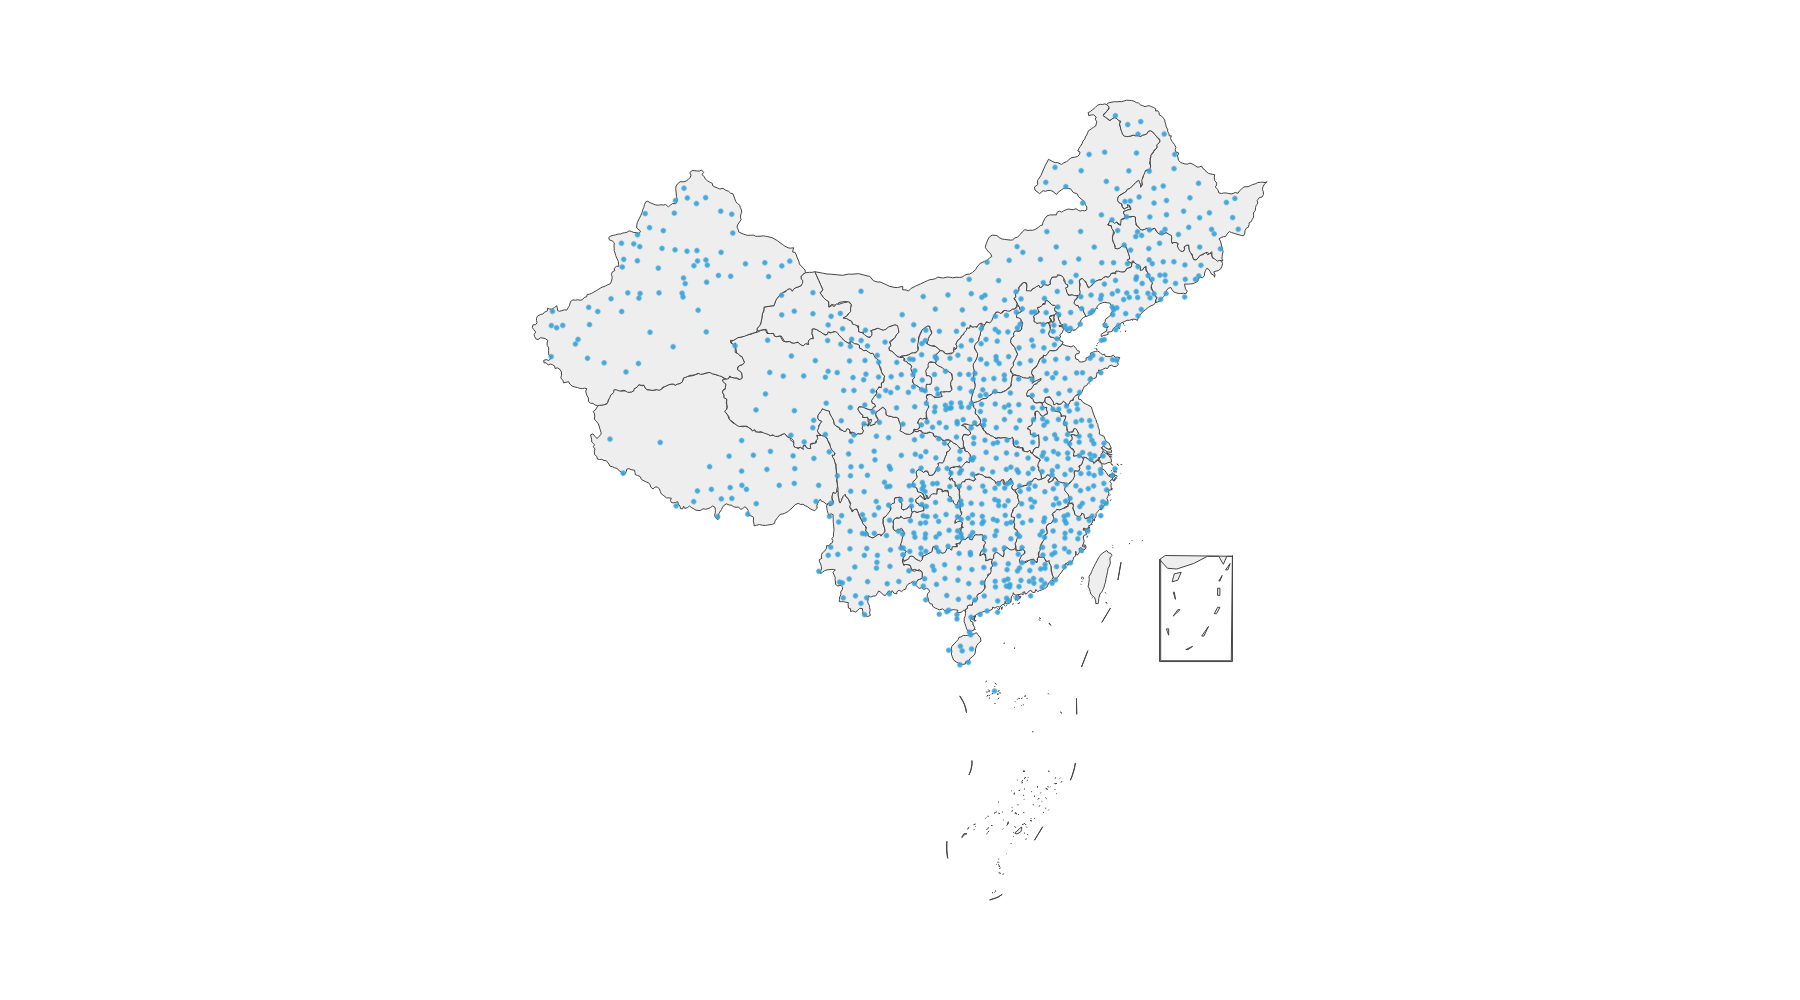
\includegraphics[width=\textwidth, trim=200 0 200 0]{lib/img/locations.png}
        \caption{原始数据中气象站的地理位置分布}
        \label{fig:location}
    \end{minipage}
    \begin{minipage}{0.48\linewidth}
        \includegraphics[width=\textwidth, trim=200 0 200 0]{lib/img/near.png}
        \caption{划分为灾区气象站的地理位置分布}
    \end{minipage}
    \begin{minipage}{0.48\linewidth}
        \includegraphics[width=\textwidth, trim=200 0 200 0]{lib/img/middle.png}
        \caption{划分为近灾区气象站的地理位置分布}
    \end{minipage}
    \begin{minipage}{0.48\linewidth}
        \includegraphics[width=\textwidth, trim=200 0 200 0]{lib/img/far.png}
        \caption{划分为非灾区气象站的地理位置分布}
    \end{minipage}
\end{figure}

进一步的数据处理流程包括:首先,我们对连续变量进行了缩尾处理,即在数据的首尾1\%处进行了截断。其次,为了确保气象数据与保单数据之间的相关性,我们对选取的保单进行了地理限制,只选择了那些距离最近的监测站20公里以内的保单进行分析。这样的限制有助于确保气象数据与保单之间的相关性更加紧密,因为气象条件对保险赔付的影响往往与地理位置密切相关。

在完成了上述数据处理步骤后,本文最终将1914万条气象数据与610万条保单数据进行了匹配,得到约了70万条可用于回归分析的数据。

\section{模型设定与变量定义}

极端天气事件是一个外生冲击,在时空上的分布是随机的,因此本文采用了DID回归来估计极端天气事件对家庭财产保险的影响。DID回归的基本思想是通过对照组和实验组的比较,消除了时间不变的个体特征对估计结果的影响,从而更加准确地估计政策的效果。本文设定了一个虚拟的实验组和对照组,实验组为受灾区或近灾区,对照组为未受灾区,通过比较两组在巨灾发生前后的差异来估计极端天气事件对财产保险的影响。

本文采用的主要被解释变量为家财险保额,反映家庭对财产保险的需求。而主要解释变量为极端天气事件的虚拟变量,分为两个维度:一是是否受灾,即家庭所在地区是否直接遭受了极端天气事件的影响;二是是否邻近灾区,即使家庭所在地区未直接受灾,但若邻近地区遭受灾害,也可能会影响他们的保险需求。

此外,为了更全面地评估极端天气事件的影响,本文纳入一系列控制变量。这些变量包括:
\begin{enumerate}
    \item 是否历史投保:反映了家庭过去的保险购买行为,可能影响他们对未来保险需求的决策。
    \item 保险财产购置价:反映了家庭财产的价值,通常财产价值越高,保险需求也越大。
    \item 建筑面积:建筑面积越大,需要更高的保险保额来覆盖潜在的风险。
\end{enumerate}

\begin{table}[H]
    \caption{变量定义表}\label{tab:var}
    \begin{tabular}{@{}cccc@{}}
        \toprule
        变量类别                    & 变量名称    & 变量定义   & 解释           \\ \midrule
        被解释变量                   & Coverage    & 保额      & 保险金额    \\ \midrule
        \multirow{3}{*}{主要解释变量} & Disaster    & 灾区      & 是否处于极端降水监测点20公里内    \\ \cmidrule(l){2-4}
                                & Neighbor    & 近灾区     & 是否处于极端降水监测点20-50公里内 \\ \cmidrule(l){2-4}
                                & Post        & 是否投保    &  是否在极端降水发生后投保                 \\ \midrule
        \multirow{4}{*}{控制变量}   & Prem\_before & 历史投保    & 保险标的是否有投保记录        \\ \cmidrule(l){2-4}
                                & Price       & 保险财产购置价 & 保险标的资产购置价            \\ \cmidrule(l){2-4}
                                & Area        & 建筑面积    & 保险标的建筑面积                  \\ \cmidrule(l){2-4}
                                & Claim       & 是否理赔    & 该保单是否发生理赔            \\ \bottomrule
    \end{tabular}
\end{table}


考虑保额分布有下界不满足正态分布,因此针对假设H\ref{hyp:1}本文的OLS模型如下:
\begin{equation}
    \log\text{Coverage}=\alpha+\beta_1\text{Post}+\beta\text{Controls}+\varepsilon
    \label{eq:OLS}
\end{equation}

而针对假设H\ref{hyp:2}本文的DID模型如下:

\begin{equation}
    \log\text{Coverage}=\alpha+\beta_1\text{Disaster}+\beta_2\text{Post}+\beta_3\text{Disaster}\times\text{Post}+\beta\text{Controls}+\varepsilon
    \label{eq:DID_1}
\end{equation}

而针对假设H\ref{hyp:3}本文的DID模型如下:

\begin{equation}
    \log\text{Coverage}=\alpha+\beta_1\text{Neighbor}+\beta_2\text{Post}+\beta_3\text{Neighbor}\times\text{Post}+\beta\text{Controls}+\varepsilon
    \label{eq:DID_2}
\end{equation}


\chapter{实证结果与分析}\label{chap:4}
\section{描述性统计}
TODO:fix数据
主要变量的描述性统计结果如表\ref{tab:desc}所示。保额Coverage的均值为514,139.56元,保费Premium的均值为1,175.71元,保险标的购置价Price均值为0.61百万元。是否此前投保(Prem\_before)的均值为0.04,标准差为0.20。监测站点和保险标的的地理位置距离(distance)的均值为13.24公里,标准差为4.46,表明观测点之间的距离相对集中。累计降水量(累计降水量)的均值为2,042.35,标准差为712.30,显示了不同观测点之间降水量的变异性。
% 表\ref{tab:corr}报告了主要变量的相关系数矩阵,变量相关系数极低,说明本文的实证研究结果不存在多重共线性。

\begin{table}[H]
    \caption{数据描述性统计}\label{tab:desc}
    \centering
    \begin{tabular}{lrrrrrr}
    \toprule
    变量名         & 观测数    & 均值        & 标准差       & 最小值      & 中位数       & 最大值        \\
    \midrule
    Coverage    & 368908 & 294652.92 & 323379.27 & 20092.78 & 200000.00 & 2991900.00 \\
    Price       & 368908 & 48.26     & 50.30     & 0.00     & 31.40     & 371.84     \\
    GDP         & 368908 & 0.17      & 0.04      & 0.07     & 0.18      & 0.24       \\
    Density     & 368908 & 236.56    & 156.53    & 37.78    & 184.32    & 821.75     \\
    Penetration & 368908 & 0.79      & 0.16      & 0.45     & 0.80      & 1.20       \\
    distance    & 368908 & 13.27     & 4.61      & 0.26     & 14.06     & 20.00      \\
    Premium     & 368908 & 1028.88   & 1031.51   & 10.20    & 661.50    & 5550.00    \\
    累计赔付额       & 454    & 27556.84  & 73421.40  & 10.00    & 1477.50   & 517183.53  \\
    保费          & 368908 & 1028.88   & 1031.51   & 10.20    & 661.50    & 5550.00    \\
    极端降水量       & 268484 & 410.12   & 117.58    & 51.40   & 388.00   & 595.00    \\
    \bottomrule
\end{tabular}

\end{table}

TODO:
图xx显示了

\begin{figure}[H]
    \begin{minipage}{0.48\linewidth}
        \includegraphics[width=\linewidth]{lib/img/olsdistance.png}
        \caption{标的与监测站距离分布}
    \end{minipage}
    \begin{minipage}{0.48\linewidth}
        \includegraphics[width=\linewidth]{lib/img/coverage.png}
        \caption{标的保额对数分布}
    \end{minipage}
\end{figure}
\begin{figure}[H]
    \begin{minipage}{0.48\linewidth}
        \includegraphics[width=\linewidth]{img/insurance.png}
        \caption{保险标的保险起期分布}
    \end{minipage}
    \begin{minipage}{0.48\linewidth}
        \includegraphics[width=\linewidth]{lib/img/precip.png}
        \caption{灾区家庭经历极端降水量的对数分布}
        TODO:对齐图,用没取对数的
    \end{minipage}
\end{figure}
% 截止2012年7月22日凌晨2时,北京全市平均降雨量164毫米,城区平均降雨量212毫米,降雨最大点在房山区河北镇,降雨量519毫米。
% \begin{table}[H]
%     \caption{变量之间相关性}\label{tab:corr}
%     \centering
%     \begin{tabular}{lrrrrrrr}
\toprule
 & Coverage & Disaster & Neighbor & Post & Prem\_before & Price & Area \\
\midrule
Coverage & 1.000000 & -0.003438 & 0.002232 & 0.006549 & 0.049063 & 0.195955 & -0.000131 \\
Disaster & -0.003438 & 1.000000 & -0.112619 & -0.199710 & -0.031179 & -0.027510 & -0.000619 \\
Neighbor & 0.002232 & -0.112619 & 1.000000 & -0.025723 & 0.004791 & 0.002799 & -0.000466 \\
Post & 0.006549 & -0.199710 & -0.025723 & 1.000000 & 0.014869 & 0.023873 & 0.000746 \\
Prem\_before & 0.049063 & -0.031179 & 0.004791 & 0.014869 & 1.000000 & 0.080722 & -0.000330 \\
Price & 0.195955 & -0.027510 & 0.002799 & 0.023873 & 0.080722 & 1.000000 & -0.000173 \\
Area & -0.000131 & -0.000619 & -0.000466 & 0.000746 & -0.000330 & -0.000173 & 1.000000 \\
\bottomrule
\end{tabular}


% \end{table}

\section{基准回归结果}
% \subsection{模型\ref{eq:OLS}:基础回归}
% 对于假设\ref{hyp:1},回归结果见表\ref{tab:ols}。

% \begin{table}[htbp]
%     \centering
%     \caption{OLS回归结果}\label{tab:ols}
%     
\begin{tabular}{@{\extracolsep{5pt}}lcc}
\\[-1.8ex]\hline
\hline \\[-1.8ex]
& \multicolumn{2}{c}{\textit{Dependent variable: log(Coverage)}} \
\cr \cline{2-3}
\\[-1.8ex] & (1) & (2) \\
\hline \\[-1.8ex]
 Area & & -0.000$^{}$ \\
& & (0.000) \\
 Intercept & 12.265$^{***}$ & 12.158$^{***}$ \\
& (0.004) & (0.003) \\
 Post & 0.100$^{***}$ & 0.071$^{***}$ \\
& (0.004) & (0.004) \\
 Prem\_before & & 0.670$^{***}$ \\
& & (0.008) \\
 Price & & 0.136$^{***}$ \\
& & (0.001) \\
\hline \\[-1.8ex]
 Observations & 414961 & 414961 \\
 $R^2$ & 0.001 & 0.171 \\
 Adjusted $R^2$ & 0.001 & 0.171 \\
 Residual Std. Error & 1.021 (df=414959) & 0.930 (df=414956) \\
 F Statistic & 584.020$^{***}$ (df=1; 414959) & 21392.415$^{***}$ (df=4; 414956) \\
\hline
\hline \\[-1.8ex]
\textit{Note:} & \multicolumn{2}{r}{$^{*}$p$<$0.1; $^{**}$p$<$0.05; $^{***}$p$<$0.01} \\
\end{tabular}

% \end{table}

\subsection{近灾区的DID回归}
对于假设\ref{hyp:3},回归结果见表\ref{tab:did1}。回归结果显示,在控制了其他变量之后,近灾区的交互项$\text{Neighbor}\times \text{Post}$的系数显著为正,这一结果验证了假设\ref{hyp:3},意味着在极端天气事件发生后,近灾区的保额提升了约23\%。近灾区居民由于接收到更丰富的信息,对极端天气事件的敏感度增强,因此他们的保险需求也相应增加。这种信息的丰富性可能来自于更直接的灾害经历、媒体报道、社区讨论等多种渠道,使得近灾区居民对灾害的潜在影响有了更深刻的认识。
\begin{table}[H]
    \centering
    \caption{实验组为近灾区的DID回归结果}\label{tab:did1}
    
\begin{tabular}{@{\extracolsep{5pt}}lcc}
\\[-1.8ex]\hline
\hline \\[-1.8ex]
& \multicolumn{2}{c}{\textit{Dependent variable: log(Coverage)}} \
\cr \cline{2-3}
\\[-1.8ex] & (1) & (2) \\
\hline \\[-1.8ex]
 Area & & -0.000$^{}$ \\
& & (0.000) \\
 Intercept & 12.164$^{***}$ & 12.067$^{***}$ \\
& (0.005) & (0.004) \\
 Neighbor & 0.227$^{***}$ & 0.224$^{***}$ \\
& (0.013) & (0.012) \\
 Neighbor:Post & 0.086$^{***}$ & 0.087$^{***}$ \\
& (0.015) & (0.014) \\
 Post & 0.095$^{***}$ & 0.068$^{***}$ \\
& (0.005) & (0.005) \\
 Prem\_before & & 0.542$^{***}$ \\
& & (0.008) \\
 Price & & 0.153$^{***}$ \\
& & (0.001) \\
\hline \\[-1.8ex]
 Observations & 455107 & 455107 \\
 $R^2$ & 0.006 & 0.136 \\
 Adjusted $R^2$ & 0.006 & 0.136 \\
 Residual Std. Error & 1.150 (df=455103) & 1.072 (df=455100) \\
 F Statistic & 961.465$^{***}$ (df=3; 455103) & 11948.789$^{***}$ (df=6; 455100) \\
\hline
\hline \\[-1.8ex]
\textit{Note:} & \multicolumn{2}{r}{$^{*}$p$<$0.1; $^{**}$p$<$0.05; $^{***}$p$<$0.01} \\
\end{tabular}

\end{table}

此外,当极端天气事件发生(即$\text{Post=1}$)时,不论家庭是否是否位于近灾区,家财险的保额整体上提高了约10\%。这一提升是显著为正,意味着在极端天气事件的影响下,家庭的风险感知得到了加强,从而增加了他们对家财险的需求。这一发现与假设\ref{hyp:3}的预期一致,即极端天气事件通过提高风险感知,导致家财险需求的提升。

控制变量方面,回归结果还表明,在家庭层面,保险标的的购置价每提升1\%导致保额平均提升0.36\%,家庭之前投保过会导致保额平均提升24\%。这两个变量的系数显著为正,与直觉相符,即价值较高的财和有保险购买历史的家庭更倾向于购买更高额度的保险。而在地区层面,GDP增速每增加1\%,家财险的保额整体上小幅提高约0.001\%,反应经济发展水平对保险需求的正向提升作用\citep{JJYJ200401002,arena2008does};而保险深度每提升1\%,家财险的保额整体上提高约0.67\%,反应保险市场的发展对保险需求的正向提升作用\citep{JRYJ200706018}。这两个变量的系数显著为正,与保险需求与经济发展水平、保险市场发展水平正相关的理论预期一致。

% 此外,DID回归结果还揭示了近灾区与远灾区之间的差异。近灾区的系数显著为正,表明与远灾区相比,近灾区的居民在灾害发生后购买的家财险保额提升了约22\%。这一差异可能源于近灾区居民对极端降水概率的主观判断更高,因此他们的风险感知也更强。这种强烈的风险感知可能促使他们购买更高额度的保险,以更好地保护自己的财产。

\subsection{灾区的DID回归}
对于假设\ref{hyp:2},回归结果见表\ref{tab:did2}。与表\ref{tab:did1}类似,该组也验证了假设\ref{hyp:3},即极端天气事件发生后购买家财险的保额提升约10\%。但是,交互项$\text{Disaster}\times \text{Post}$的系数为负,即灾区相对非灾区在受灾后反而降低了14\%保额,完全抵消了受灾后的10\%保额增加的影响,保额反而相对降低。其他控制变量的结果与表\ref{tab:did2}基本一致,保险标的的购置价、家庭之前投保过、GDP增速、保险深度等变量的系数符号与表\ref{tab:did1}一致,且显著性水平也基本一致。

TODO: note
\begin{table}[H]
    \centering
    \caption{实验组为灾区的DID回归结果}\label{tab:did2}
    
\begin{tabular}{@{\extracolsep{5pt}}lcc}
    \\[-1.8ex]\hline
    \hline                                                                                                         \\[-1.8ex]
                         & \multicolumn{2}{c}{\textit{Dependent variable: log(Coverage)}} \
    \cr \cline{2-3}
    \\[-1.8ex] & (1) & (2) \\
    \hline                                                                                                         \\[-1.8ex]
    Disaster$\times$Post & -0.396$^{***}$                                                       & -0.187$^{***}$   \\
                         & (0.010)                                                              & (0.008)          \\
    Disaster             & 0.085$^{***}$                                                        & -0.008$^{}$      \\
                         & (0.009)                                                              & (0.007)          \\
    Post                 & 0.210$^{***}$                                                        & 0.113$^{***}$    \\
                         & (0.006)                                                              & (0.005)          \\
    Prem\_before         &                                                                      & 0.214$^{***}$    \\
                         &                                                                      & (0.007)          \\
    log(GDP)             &                                                                      & 0.102$^{***}$   \\
                         &                                                                      & (0.008)          \\
    log(Penetration)     &                                                                      & 0.699$^{***}$    \\
                         &                                                                      & (0.007)          \\
    log(Price)           &                                                                      & 0.364$^{***}$    \\
                         &                                                                      & (0.001)          \\
    Intercept            & 12.452$^{***}$                                                       & 11.460$^{***}$   \\
                         & (0.113)                                                              & (0.093)          \\
    \hline                                                                                                         \\[-1.8ex]
    Observations         & 285872                                                               & 285872           \\
    $R^2$                & 0.088                                                                & 0.407            \\
    Adjusted $R^2$       & 0.088                                                                & 0.407            \\
    Residual Std. Error  & 0.838                                                                & 0.676            \\
    F Statistic          & 1719.357$^{***}$                                                     & 9815.498$^{***}$ \\
    Year FE              & Yes                                                                  & Yes              \\
    \hline
    \hline
    \textit{Note:}       & \multicolumn{2}{r}{$^{*}$p$<$0.1; $^{**}$p$<$0.05; $^{***}$p$<$0.01}                    \\
\end{tabular}

\end{table}

\section{稳健性检验}
\subsection{平行趋势检验}

为了验证DID实证结果的稳健性,需要进行平行趋势检验。表\ref{tab:robust}展示了平行趋势检验的结果,并可视化如图\ref{fig:robust}。本文分别将实验组设置为灾区和近灾区($\text{Treat}=\text{Disaster}$以及$\text{Treat}=\text{Neighbor}$),对极端天气事件发生前四个季度的保额进行回归。回归结果显示交互项的系数都不显著,这表明在极端天气事件发生前,实验组和对照组的保额水平基本是平行的,满足平行趋势假设,可以通过DID方法来估计极端天气事件对家财险需求的影响。
% 唯一表现出显著性的部分是在灾区受灾前90天内(一个季度)的保额,这可能是因为20年一遇的极端降水往往是持续较久的,灾区居民达到20年一遇的门槛前已经开始感知到风险,从而提前购买了保险。

\begin{figure}[H]
    \includegraphics[width=\linewidth]{lib/img/robust.png}
    \caption{平行趋势检验}\label{fig:robust}
\end{figure}
\begin{table}[H]
    \centering
    \renewcommand{\arraystretch}{0.8}
    \caption{平行趋势检验}\label{tab:robust}
    
\begin{tabular}{@{\extracolsep{5pt}}lcc}
    \\[-1.8ex]\hline
    \hline                                                                                                           \\[-1.8ex]
                           & \multicolumn{2}{c}{\textit{Dependent variable: log(Coverage)}} \
    \cr \cline{2-3}
    \\[-1.8ex] & \multicolumn{1}{c}{Disaster} & \multicolumn{1}{c}{Neighbor}  \\
    \\[-1.8ex] & (1) & (2) \\
    \hline                                                                                                           \\[-1.8ex]
    Treated:C(Years)[T.-3] & -0.014$^{}$                                                          & -0.013$^{}$      \\
                           & (0.021)                                                              & (0.059)          \\
    Treated:C(Years)[T.-2] & -0.022$^{}$                                                          & -0.048$^{}$      \\
                           & (0.021)                                                              & (0.060)          \\
    Treated:C(Years)[T.-1] & -0.028$^{}$                                                          & -0.079$^{}$      \\
                           & (0.021)                                                              & (0.058)          \\
    Treated:C(Years)[T.0]  & -0.147$^{***}$                                                       & 0.185$^{***}$    \\
                           & (0.015)                                                              & (0.045)          \\
    Treated:C(Years)[T.1]  & -0.542$^{*}$                                                         & 0.218$^{***}$    \\
                           & (0.323)                                                              & (0.045)          \\
    Treated                & -0.021$^{}$                                                          & -0.202$^{***}$   \\
                           & (0.015)                                                              & (0.043)          \\
    % C(Years)[T.-1]         & 0.023$^{*}$                                                          & 0.023$^{}$       \\
    %                        & (0.014)                                                              & (0.015)          \\
    % C(Years)[T.-2]         & 0.018$^{}$                                                           & 0.018$^{}$       \\
    %                        & (0.014)                                                              & (0.015)          \\
    % C(Years)[T.-3]         & 0.001$^{}$                                                           & 0.001$^{}$       \\
    %                        & (0.014)                                                              & (0.015)          \\
    % C(Years)[T.0]          & 0.101$^{***}$                                                        & 0.109$^{***}$    \\
    %                        & (0.010)                                                              & (0.011)          \\
    % C(Years)[T.1]          & 0.111$^{***}$                                                        & 0.120$^{***}$    \\
    %                        & (0.010)                                                              & (0.011)          \\
    Intercept              & 10.764$^{***}$                                                       & 10.956$^{***}$   \\
                           & (0.015)                                                              & (0.018)          \\
    Controls                & Yes                                                                  & Yes              \\
    % Prem\_before           & 0.242$^{***}$                                                        & 0.237$^{***}$    \\
    %                        & (0.010)                                                              & (0.010)          \\
    % log(GDP)               & -0.088$^{***}$                                                       & -0.071$^{***}$   \\
    %                        & (0.006)                                                              & (0.007)          \\
    % log(Penetration)       & 0.771$^{***}$                                                        & 0.801$^{***}$    \\
    %                        & (0.008)                                                              & (0.010)          \\
    % log(Price)             & 0.416$^{***}$                                                        & 0.370$^{***}$    \\
    %                        & (0.001)                                                              & (0.002)          \\
    \hline                                                                                                           \\[-1.8ex]
    Observations           & 153904                                                               & 117647           \\
    $R^2$                  & 0.452                                                                & 0.401            \\
    Adjusted $R^2$         & 0.452                                                                & 0.401            \\
    Residual Std. Error    & 0.645                                                                & 0.689            \\
    F Statistic            & 8470.798$^{***}$                                                     & 5240.783$^{***}$ \\
    \hline
    \hline
    \textit{Note:}         & \multicolumn{2}{r}{$^{*}$p$<$0.1; $^{**}$p$<$0.05; $^{***}$p$<$0.01}                    \\
\end{tabular}

\end{table}

\subsection{安慰剂检验}
为排除其他潜在政策和遗漏变量等对回归结果的干扰,本文参考\citet{CYJJ202104009}随机虚构处理组,将 Neighbor 和 Disaster 的 DID 随机分组分配重复 500 次,结果如图\ref{fig:randomtest}所示。随机分配结果的所有系数估计值大体呈均值为 0 的正态分布,说明实验结果不是由于其他潜在政策或遗漏变量引起的,而是由于极端天气事件的影响。
\begin{figure}[H]
    \includegraphics[width=\linewidth]{lib/img/randomtest.png}
    \caption{安慰剂检验}\label{fig:randomtest}
\end{figure}

\subsection{其他稳健性检验}

为保证基准回归结果的稳健性,本文还进行了以下稳健性检验:(1)(2)更换家财险需求的度量方式为保费Premium;(3)(4)/(5)(6)参考\citet{alok2020fund}分别将灾区距离上界从 20km 改为10km。回归结果如表\ref{tab:robustdid}所示。就回归结果而言,基本与基准回归结果一致,表明本文的实证结果是稳健的。这一结果进一步验证了极端天气事件通过增强家庭的风险感知,导致家财险需求的提升。
\begin{sidewaystable}[htbp]
    \centering
    \caption{稳健性检验回归结果}\label{tab:robustdid}
    
\begin{tabular}{@{\extracolsep{5pt}}lcccccc}
\\[-1.8ex]\hline
\hline \\[-1.8ex]
\\[-1.8ex] & \multicolumn{1}{c}{log(Premium)} & \multicolumn{1}{c}{log(Premium)} & \multicolumn{1}{c}{<30km} & \multicolumn{1}{c}{<30km} & \multicolumn{1}{c}{<10km} & \multicolumn{1}{c}{<10km}  \\
\\[-1.8ex] & (1) & (2) & (3) & (4) & (5) & (6) \\
\hline \\[-1.8ex]
 Area & 0.000$^{}$ & 0.000$^{}$ & 0.000$^{}$ & 0.000$^{}$ & 0.000$^{}$ & 0.000$^{}$ \\
& (0.000) & (0.000) & (0.000) & (0.000) & (0.000) & (0.000) \\
 Disaster & & -0.149$^{***}$ & & 0.187$^{***}$ & & 0.170$^{***}$ \\
& & (0.009) & & (0.006) & & (0.011) \\
 Disaster:Post & & -0.036$^{***}$ & & -0.207$^{***}$ & & -0.277$^{***}$ \\
& & (0.011) & & (0.007) & & (0.013) \\
 Intercept & 6.257$^{***}$ & 6.255$^{***}$ & 12.052$^{***}$ & 12.055$^{***}$ & 12.086$^{***}$ & 12.106$^{***}$ \\
& (0.005) & (0.005) & (0.003) & (0.003) & (0.006) & (0.006) \\
 Neighbor & 0.065$^{***}$ & & 0.222$^{***}$ & & 0.158$^{***}$ & \\
& (0.013) & & (0.012) & & (0.014) & \\
 Neighbor:Post & 0.024$^{}$ & & 0.150$^{***}$ & & 0.209$^{***}$ & \\
& (0.015) & & (0.013) & & (0.016) & \\
 Post & 0.097$^{***}$ & 0.097$^{***}$ & -0.000$^{}$ & -0.000$^{}$ & 0.085$^{***}$ & 0.098$^{***}$ \\
& (0.005) & (0.005) & (0.003) & (0.003) & (0.002) & (0.002) \\
 Prem\_before & -0.801$^{***}$ & -0.785$^{***}$ & 0.574$^{***}$ & 0.576$^{***}$ & 0.386$^{***}$ & 0.395$^{***}$ \\
& (0.009) & (0.009) & (0.006) & (0.006) & (0.009) & (0.010) \\
 Price & 0.084$^{***}$ & 0.086$^{***}$ & 0.184$^{***}$ & 0.178$^{***}$ & 0.238$^{***}$ & 0.198$^{***}$ \\
& (0.001) & (0.001) & (0.001) & (0.001) & (0.001) & (0.001) \\
\hline \\[-1.8ex]
 Observations & 408439 & 433025 & 853757 & 939148 & 270762 & 277046 \\
 $R^2$ & 0.041 & 0.038 & 0.150 & 0.131 & 0.190 & 0.146 \\
 Adjusted $R^2$ & 0.041 & 0.038 & 0.150 & 0.131 & 0.190 & 0.146 \\
 Residual Std. Error & 1.138  & 1.143  & 1.076  & 1.098  & 1.022  & 1.065  \\
 F Statistic & 2885.524$^{***}$  & 2880.383$^{***}$  & 25027.608$^{***}$  & 23637.295$^{***}$  & 10588.824$^{***}$  & 7863.860$^{***}$  \\
\hline
\hline \\[-1.8ex]
\textit{Note:} & \multicolumn{6}{r}{$^{*}$p$<$0.1; $^{**}$p$<$0.05; $^{***}$p$<$0.01} \\
\end{tabular}

\end{sidewaystable}

具体而言,表\ref{tab:robustdid}的模型(1)(2)显示,当极端天气事件发生后,家庭的保费整体上提高了约5\%。这一提升是显著为正,意味着在极端天气事件的影响下,家庭的风险感知得到了加强,从而增加了他们对家财险的需求。这一发现与假设\ref{hyp:3}的预期一致,即极端天气事件通过提高风险感知,导致家财险需求的提升。但灾区交互项的系数为负,表明灾区的保费在受灾后反而降低了约16\%,近灾区则提升了约57\%,与假设\ref{hyp:3}、假设\ref{hyp:2}一致。

就更改距离而言,模型(3)(4)/(5)(6)分别更改灾区受灾半径的上界至10km/30km,整体而言并不会改变实证结果,同样显示出灾区灾后保额购买减少约10-15\%、近灾区保额购买提升25-30\%,表明本文的实证结果是稳健的。

%!root = ../main.tex
\chapter{扩展问题的实证结果}\label{chap:4.1}
在基础回归的基础上,本文将在基准回归的基础上进行进一步的异质性分析,主要通过探讨两个问题:第一,地区之间的异质性效应是否仅限于与灾区的相对位置关系,还是也包括它们的绝对地理位置?第二,对于极端天气事件的反应是否仅与事件发生的相对时间有关,还是不同绝对时间点的反应也存在显著差异。本文将分别对这两个问题进行实证分析。

\section{地区异质性分析:适应性预期造成灾区结果差异}
在探讨极端天气事件对不同地区影响的差异性时,本文首先关注了地区对此类事件的反应是否存在显著的地域性差异。基于东部沿海地区频繁遭受降水事件的影响,居民可能因多次面对风险而逐渐形成了对此类风险的适应性预期。正如台风路径上的企业对自然灾害的反应效率提升\citep{0Do},频繁的降水可能为他们累积了经验,降低了对极端天气的敏感度\citep{陈思柳2021不同决策情境下的损失厌恶效应差异}。
相反,在干旱少雨的西部地区,由于降水事件较为罕见,由于降水相对较少对极端降水风险的敏感度不足,这可能导致他们在面对极端天气时的反应与东部地区存在显著差异。

为了验证这一假设,本研究根据国家统计局的划分标准,将样本划分为东部、中部和西部三个地区,并分别进行了回归分析。回归结果如表\ref{tab:het_geo}所示,基本与表\ref{tab:did1}和表\ref{tab:did2}一致。东部和中部地区在遭受极端降水事件后,所有地区的保险金额均有显著增长;然而,在灾区,交互项系数为负,表明保险金额有所下降,而在近灾区,保险金额的增长更为显著。

\begin{sidewaystable}[htbp]
    \centering
    \caption{分地区回归结果}\label{tab:het_geo}
    
\begin{tabular}{@{\extracolsep{5pt}}lcccccc}
\\[-1.8ex]\hline
\hline \\[-1.8ex]
& \multicolumn{6}{c}{\textit{Dependent variable: log(Coverage)}} \
\cr \cline{2-7}
\\[-1.8ex] & \multicolumn{1}{c}{East} & \multicolumn{1}{c}{Middle} & \multicolumn{1}{c}{West} & \multicolumn{1}{c}{East} & \multicolumn{1}{c}{Middle} & \multicolumn{1}{c}{West}  \\
\\[-1.8ex] & (1) & (2) & (3) & (4) & (5) & (6) \\
\hline \\[-1.8ex]
 Disaster & -0.090$^{***}$ & 0.054$^{***}$ & -0.159$^{***}$ & & & \\
& (0.006) & (0.008) & (0.006) & & & \\
 Disaster:Post & -0.121$^{***}$ & -0.136$^{***}$ & 0.123$^{***}$ & & & \\
& (0.007) & (0.009) & (0.008) & & & \\
 Neighbor & & & & -0.233$^{***}$ & -0.136$^{***}$ & -0.490$^{***}$ \\
& & & & (0.016) & (0.018) & (0.129) \\
 Neighbor:Post & & & & 0.246$^{***}$ & 0.052$^{***}$ & 0.570$^{***}$ \\
& & & & (0.017) & (0.019) & (0.129) \\
 Post & 0.065$^{***}$ & 0.036$^{***}$ & -0.171$^{***}$ & 0.065$^{***}$ & 0.037$^{***}$ & -0.172$^{***}$ \\
& (0.004) & (0.004) & (0.004) & (0.004) & (0.004) & (0.004) \\
%  Prem\_before & 0.185$^{***}$ & 0.107$^{***}$ & 0.067$^{***}$ & 0.174$^{***}$ & 0.106$^{***}$ & 0.071$^{***}$ \\
% & (0.006) & (0.030) & (0.016) & (0.006) & (0.034) & (0.016) \\
%  log(GDP) & 0.000$^{}$ & 0.000$^{}$ & -0.000$^{}$ & 0.000$^{}$ & 0.000$^{}$ & -0.000$^{}$ \\
% & (0.000) & (0.000) & (0.000) & (0.000) & (0.000) & (0.000) \\
%  log(Penetration) & 0.906$^{***}$ & 0.029$^{***}$ & 0.071$^{***}$ & 0.909$^{***}$ & 0.027$^{***}$ & 0.116$^{***}$ \\
% & (0.005) & (0.007) & (0.005) & (0.005) & (0.008) & (0.005) \\
%  log(Price) & 0.312$^{***}$ & 0.684$^{***}$ & 0.848$^{***}$ & 0.296$^{***}$ & 0.672$^{***}$ & 0.852$^{***}$ \\
% & (0.001) & (0.002) & (0.001) & (0.001) & (0.002) & (0.002) \\
Intercept & 11.386$^{***}$ & 9.757$^{***}$ & 9.331$^{***}$ & 11.444$^{***}$ & 9.793$^{***}$ & 9.298$^{***}$ \\
& (0.005) & (0.006) & (0.007) & (0.006) & (0.007) & (0.007) \\
Controls & True & True & True & True & True & True \\
\hline \\[-1.8ex]
 Observations & 481063 & 123513 & 104695 & 450350 & 107232 & 96922 \\
 $R^2$ & 0.333 & 0.593 & 0.764 & 0.314 & 0.585 & 0.774 \\
 Adjusted $R^2$ & 0.333 & 0.592 & 0.764 & 0.314 & 0.585 & 0.774 \\
 Residual Std. Error & 0.704  & 0.439  & 0.375  & 0.718  & 0.447  & 0.364  \\
 F Statistic & 34345.705$^{***}$  & 25654.772$^{***}$  & 48356.638$^{***}$  & 29449.242$^{***}$  & 21634.683$^{***}$  & 47450.879$^{***}$  \\
    Year FE & True & True & True & True & True & True \\
\hline
\hline \\[-1.8ex]
\textit{Note:} & \multicolumn{6}{r}{$^{*}$p$<$0.1; $^{**}$p$<$0.05; $^{***}$p$<$0.01} \\
\end{tabular}

\end{sidewaystable}

然而,在西部地区,极端降水事件对远灾区的影响不显著,近灾区的交互项显著性较低,而灾区的交互项系数则显著为正,这与东部和中部地区的情况形成了鲜明对比。原因可能有两方面:一方面由于西部地区极端降水事件虽然也是二十年一遇,但绝对值相对较低,如图\ref{fig:rainings}所示,风险造成的损失相对有限,因此对居民行为的影响有限,导致远灾区和近灾区的显著性不高,同时回归的数值也相对较小。
另一方面,西部地区居民对极端降水风险的敏感度较低,容易低估了极端天气发生的概率\citep{tversky1973availability},导致保险覆盖不足。因此,在巨灾发生后,他们可能有补充保障的动机,这反映在灾区交互项系数显著为正上。

综上所述,本研究的结果揭示了不同地区对极端天气事件的反应确实存在显著的地域性差异。这种差异可能源于地区间对极端天气风险感知程度的不同,进而导致了不同的保险需求水平。但总的来说,这一发现与假设H\ref{hyp:1}的预期保持一致,即极端天气事件本质上是通过提高风险感知,导致家财险需求的增加

\begin{figure}[htbp]
    \centering
    \begin{minipage}{0.48\linewidth}
        \includegraphics[width=\linewidth]{lib/img/rainings.png}
        \caption{样本中西部地区二十年一遇极端降水事件降水绝对值相对偏低}\label{fig:rainings}
    \end{minipage}
    \begin{minipage}{0.48\linewidth}
        \includegraphics[width=\linewidth]{lib/img/covbyregion.png}
        \caption{西部地区在极端降水发生后有补充保险保障的动机}
    \end{minipage}
\end{figure}
\section{时间异质性分析:地震巨灾造成近灾区结果差异}
在探讨极端天气事件对不同时间点的反应差异时,本文以2008年为界,将样本最丰富的时间段分割为2003-2008年和2009-2013年两段,分别代表了两个不同的经济时期,得到的回归结果如表\ref{tab:het_time}所示,也与表\ref{tab:did1}和表\ref{tab:did2}基本一致,即表现为极端天气事件发生后控制组购买家财险的保额普遍提升,但灾区提升相对有限。

值得注意的是,近灾区交互项在2008年后显示出很强的正向提升,这可能是由于2008年汶川大地震使得居民对家庭所在周边的环境更为关注,对极端天气事件的风险感知提升,从而增加了对家财险的需求。这一发现也与假设H\ref{hyp:1}的预期一致,即极端天气事件通过提高风险感知从而增加家财险需求。
\begin{table}[htbp]
    \centering
    \caption{分时间回归结果}\label{tab:het_time}
    
\begin{tabular}{@{\extracolsep{5pt}}lcccc}
\\[-1.8ex]\hline
\hline \\[-1.8ex]
& \multicolumn{4}{c}{\textit{Dependent variable: log(Coverage)}} \
\cr \cline{2-5}
\\[-1.8ex] & \multicolumn{1}{c}{2003-2008} & \multicolumn{1}{c}{2009-2013} & \multicolumn{1}{c}{2003-2008} & \multicolumn{1}{c}{2009-2013}  \\
\\[-1.8ex] & (1) & (2) & (3) & (4) \\
\hline \\[-1.8ex]
 Disaster & 0.006$^{}$ & 0.004$^{}$ & & \\
& (0.006) & (0.005) & & \\
 Disaster:Post & -0.220$^{***}$ & -0.051$^{***}$ & & \\
& (0.007) & (0.006) & & \\
 Neighbor & & & -0.111$^{***}$ & -0.119$^{***}$ \\
& & & (0.015) & (0.016) \\
 Neighbor:Post & & & 0.113$^{***}$ & 0.203$^{***}$ \\
& & & (0.016) & (0.017) \\
 Post & 0.134$^{***}$ & 0.011$^{***}$ & 0.146$^{***}$ & 0.033$^{***}$ \\
% & (0.004) & (0.003) & (0.004) & (0.004) \\
%  Prem\_before & 0.215$^{***}$ & 0.039$^{***}$ & 0.210$^{***}$ & 0.025$^{***}$ \\
% & (0.007) & (0.005) & (0.006) & (0.006) \\
%  log(GDP) & 0.001$^{***}$ & 0.001$^{***}$ & 0.002$^{***}$ & 0.001$^{***}$ \\
% & (0.000) & (0.000) & (0.000) & (0.000) \\
%  log(Penetration) & 0.852$^{***}$ & 0.008$^{*}$ & 0.811$^{***}$ & -0.025$^{***}$ \\
% & (0.005) & (0.004) & (0.005) & (0.006) \\
%  log(Price) & 0.299$^{***}$ & 0.891$^{***}$ & 0.307$^{***}$ & 0.899$^{***}$ \\
% & (0.001) & (0.001) & (0.001) & (0.001) \\
Intercept & 11.270$^{***}$ & 9.124$^{***}$ & 11.219$^{***}$ & 9.109$^{***}$ \\
& (0.005) & (0.005) & (0.005) & (0.006) \\
Controls & True & True & True & True \\
\hline \\[-1.8ex]
 Observations & 479866 & 226846 & 505321 & 147024 \\
 $R^2$ & 0.314 & 0.788 & 0.314 & 0.789 \\
 Adjusted $R^2$ & 0.314 & 0.788 & 0.314 & 0.789 \\
 Residual Std. Error & 0.695  & 0.367  & 0.698  & 0.366  \\
 F Statistic & 31426.890$^{***}$  & 120172.233$^{***}$  & 33000.866$^{***}$  & 78734.049$^{***}$  \\
\hline
\hline \\[-1.8ex]
\textit{Note:} & \multicolumn{4}{r}{$^{*}$p$<$0.1; $^{**}$p$<$0.05; $^{***}$p$<$0.01} \\
\end{tabular}

\end{table}

\chapter{结论与建议}\label{chap:5}

\section{研究结论}
本研究旨在探讨极端天气事件对家庭财产保险需求的影响,以及人们的风险偏好在极端天气事件影响下的变化。通过实证分析极端降水对家财险需求的影响,本文深入探究了极端天气事件对家庭风险偏好的影响机制,填补了现有研究的空白。本文的研究结果表明,极端天气事件的发生显著提高了居民的风险感知,从而促进了家财险需求的增加。具体来说,本文的实证分析验证了以下三个研究假设:

\begin{enumerate}
    \item \textbf{假设\ref{hyp:1}}:发生极端天气事件后,居民风险感知增加,风险偏好显著提升,表现为对家财险需求的增加。OLS回归结果显示,在控制了其他变量之后,当极端天气事件发生时,家财险的保额整体上提高了约7\%,这一提升是显著为正的。
    \item \textbf{假设\ref{hyp:3}}:发生极端天气事件后,临近灾区的地区对风险厌恶增加显著,家财险需求显著增加。DID回归分析揭示了近灾区与远灾区之间的差异,近灾区的居民在灾害发生后购买的家财险保额提升了约22\%,这一差异可能源于近灾区居民对极端降水概率的主观判断更高,因此他们的风险感知也更强。
    \item \textbf{假设\ref{hyp:2}}:发生极端天气事件后,直接受到极端天气事件冲击的地区对风险偏好影响有限,家财险需求并未显著增加。DID回归结果显示,灾区相对非灾区在受灾后几乎没有增加保额,这可能是由于居民对灾害的直观感受和对保险赔付能力的初步判断所驱动的。
\end{enumerate}

\section{政策建议}
\subsection{保险公司视角:产品创新、动态定价与资本充足}
面对全球气候变化带来的挑战,极端天气事件的频发已成为不容忽视的现象。在这样的背景下,保险公司必须采取更加主动和创新的策略,以应对这些不可预测的风险。产品设计与创新是保险公司应对极端天气事件的关键领域,它要求公司不仅要关注当前的市场需求,还要预见未来可能的变化趋势。保险公司应当深入研究不同地区的气候特征和极端天气事件的类型,以便开发出更加精准和定制化的保险产品。例如,针对沿海地区频繁遭受台风侵袭的特点,可以设计包含台风风险覆盖的家财险产品;对于内陆干旱频发的区域,则可以提供针对干旱导致的财产损失的保险方案。此外,保险公司还可以开发综合性保险计划,将多种极端天气风险纳入保障范围,为客户提供一站式的风险解决方案。通过这些创新举措,保险公司不仅能够更好地满足家庭客户对于保险保障的多样化和个性化需求,还能在激烈的市场竞争中脱颖而出。创新的保险产品能够吸引更多的客户,提高客户满意度和忠诚度,从而为保险公司带来更大的市场份额和更高的收益。同时,这些产品也有助于提升保险公司的品牌形象,树立其作为行业领导者的地位,展现其对社会责任和可持续发展的承诺。

在定价策略上,保险公司必须采取更为灵活和动态的方法。保费的定价应充分考虑极端天气事件的潜在概率和损失,利用实时天气数据和气候变化趋势来调整费率。这种动态定价机制有助于确保保费收入与潜在赔付风险之间的平衡,同时也能提高保险产品的吸引力和市场适应性。

为了应对极端天气事件带来的挑战,保险公司需要在风险管理和资本充足性方面投入更多资源。加强巨灾风险管理和资本储备,参与共保和再保险机制,这些都是提高保险公司赔付能力和分散风险的有效途径。保险公司应采取更为审慎的风险评估和资本管理策略,以确保在面对极端天气事件时具备足够的财务稳定性。
\subsection{政府视角:对保障不足的潜在灾区提供补贴}

在应对极端天气事件及其对家庭财产带来的潜在威胁方面,政府和监管机构的作用不可或缺。他们不仅是规则的制定者和监督者,更是市场健康发展的推动者。当灾区保障不足时,通过实施一系列政策措施,政府可以有效促进保险业的发展,提高公众对保险产品的认知和接受度,进而增强社会整体的风险抵御能力。

首先,政府可以通过税收优惠政策,为购买家财险的家庭提供经济激励。例如,允许家庭在计算应纳税所得时扣除一定比例的保险费用,或者为购买特定极端天气风险保险产品的纳税人提供税收减免。这些措施能够降低家庭购买保险的直接成本,从而激发他们购买保险的意愿。

其次,政府可以提供补贴,特别是对于低收入家庭或高风险区域的居民,以确保他们也能够获得必要的保险保障。这些补贴可以是直接的财政支持,也可以是通过降低保险费率的方式间接提供。这样的措施有助于缩小保险覆盖的不平等差距,确保所有家庭都能在面对极端天气时得到一定程度的保护。

此外,政府和监管机构应当致力于营造一个公平、透明且竞争充分的保险市场环境。这包括简化市场准入流程,鼓励新保险公司的成立,以及支持现有保险公司开发创新产品。同时,政府还应加强对保险产品的监管,确保产品质量,保护消费者的权益。

\subsection{学术研究视角:跨领域开放数据}
为了更准确地评估和应对极端天气事件的风险,政府、保险公司和科研机构之间的数据共享与研究合作至关重要。在当前全球气候变化的大背景下,极端天气事件的不确定性和复杂性要求政府、保险公司和科研机构之间建立紧密的数据共享和研究合作关系。这种多领域、跨学科的合作模式对于提高对极端天气事件风险的评估精度和应对能力至关重要。通过跨学科的合作,结合气象学、保险学、经济学等领域的专业知识,可以更深入地理解气候变化对保险业的长期影响,并促进更有效的风险管理和保险产品创新。这种合作将为保险业提供宝贵的洞察力,帮助制定更为科学和前瞻性的风险管理策略。
% \section{研究局限与未来方向}

% 尽管本研究取得了一定的成果,但仍存在一些局限性。首先,本研究主要关注了极端降水事件对家财险需求的影响,未来研究可以扩展到其他类型的极端天气事件。其次,本研究的数据来源于特定保险公司,尽管数据量很大,但仍可能存在样本选择偏差。未来的研究可以考虑使用更广泛的数据集,以增强研究结果的普遍性。最后,本研究主要从风险感知的角度分析了极端天气事件对保险需求的影响,未来研究可以进一步探讨其他可能的影响机制,如心理预期、经济状况等因素。


\appendix
\nocite{*}
\printbibliography[heading = bibintoc, title = {参考文献}]
% \include{chap/encl1}
\backmatter
\ifblind\else%!TEX root = ../thesis.tex
\chapter{致谢}

本想总结一下大学四年,临了欲说还休。删删改改,回忆往昔,忽而想到《诗经》中的“所谓伊人”,行遍险阻,回首“宛在水中央”,便释然了。唯有最质朴的语言才能表现出最真挚的情感,或许最简单的话才能表现此刻的感受吧。

感谢我的导师刘新立副教授,感谢她平时授课时的传道授业解惑,在我写论文时的悉心指导。

感谢我在实习时导师,使我对债券市场的运作有所了解,给予我很大启发。

感谢开源以及自由软件运动的人们,使我对计算机科学产生的兴趣坚持了下去。本文的写作、编码也都是在 GPL 套件上完成的。

感谢我的父母,是我最坚实的后盾,大恩难谢。

最后也感谢自己,在目前为止最艰难的时候都挺了过来没有放弃。
\fi
\include{chap/origin}
\end{document}
